\documentclass[tikz]{standalone}
\usepackage{tikz}

\usetikzlibrary{positioning}
\usetikzlibrary{fit}
\usetikzlibrary{shapes}
\usetikzlibrary{arrows}

\tikzstyle{X} = [circle,draw,minimum size=0cm]
\tikzstyle{F} = [circle,draw,minimum size=0cm,dashed]

% Observed node
\tikzstyle{Y} = [X,fill=gray!25]


\begin{document}
	
	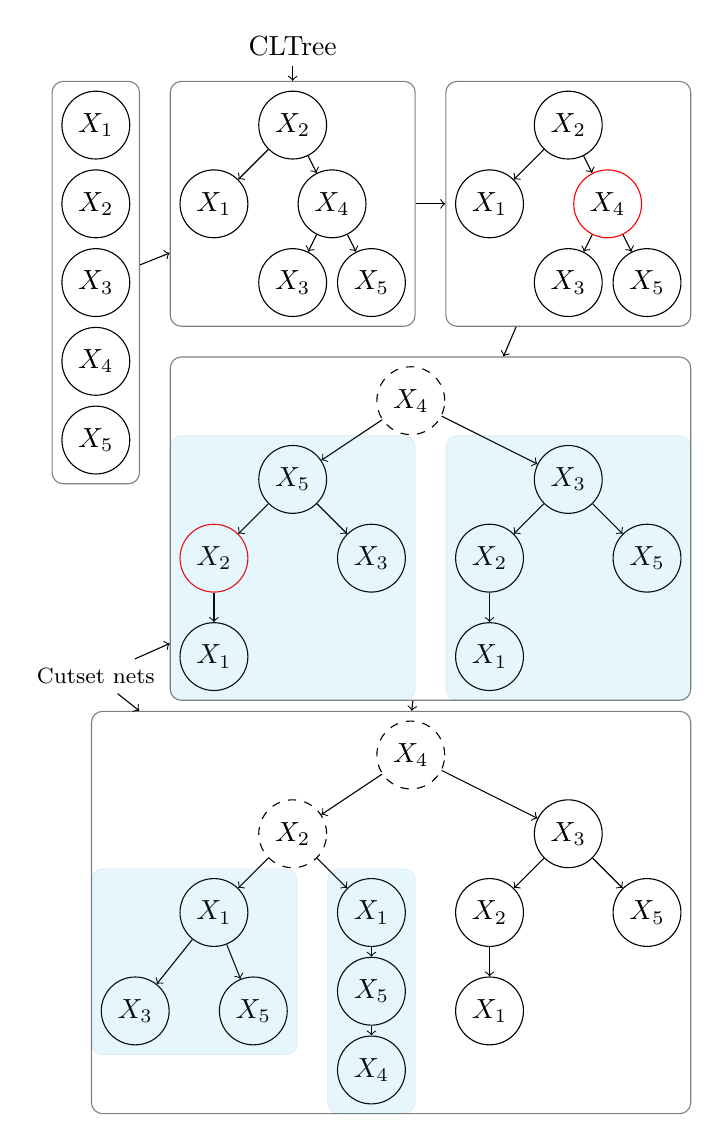
\begin{tikzpicture}
	
	
	
	\node [X] (1) at(0,0) {$X_1$};
	\node [X] (2) at(0,-1) {$X_2$};
	\node [X] (3) at(0,-2) {$X_3$};
	\node [X] (4) at(0,-3) {$X_4$};
	\node [X] (5) at(0,-4) {$X_5$};
	\node [draw=gray,rectangle,rounded corners,fit=(1) (2) (3)
	(4)(5)] (r1) {};
	%%%%%%%%%%%%%%%
	\node [X] (2a) at(2.5,0) {$X_2$};
	\node [X] (1a) at(1.5,-1) {$X_1$};
	\node [X] (4a) at(3,-1) {$X_4$};
	\node [X] (3a) at(2.5,-2) {$X_3$};
	\node [X] (5a) at(3.5,-2) {$X_5$};
	\draw [->] (2a) -- (1a) ;
	\draw [->] (2a) -- (4a) ;
	\draw [->] (4a) -- (3a) ;
	\draw [->] (4a) -- (5a) ;
	\node [draw=gray,rectangle,rounded corners,fit=(1a) (2a) (3a)
	(4a)(5a)] (r2) {};
	\draw [->] (r1) -- (r2) ;
	\node [draw=none] (aa) at(2.5,1) {CLTree};
	\draw [->] (aa) -- (r2) ;
	%%%%%%%%%
	\node [X] (2a) at(6,0) {$X_2$};
	\node [X] (1a) at(5,-1) {$X_1$};
	\node [X,draw=red] (4a) at(6.5,-1) {$X_4$};
	\node [X] (3a) at(6,-2) {$X_3$};
	\node [X] (5a) at(7,-2) {$X_5$};
	\draw [->] (2a) -- (1a) ;
	\draw [->] (2a) -- (4a) ;
	\draw [->] (4a) -- (3a) ;
	\draw [->] (4a) -- (5a) ;
	\node [draw=gray,rectangle,rounded corners,fit=(1a) (2a) (3a)
	(4a)(5a)] (r3) {};
	\draw [->] (r2) -- (r3) ;
	%%%%%%%%%%%
	\node[F] (4b) at (4,-3.5){$X_4$};
	\node [X] (5b) at(2.5,-4.5) {$X_5$};
	\node [X,draw=red] (2b) at(1.5,-5.5) {$X_2$};
	\node [X] (3b) at(3.5,-5.5) {$X_3$};
	\node [X] (1b) at(1.5,-6.75) {$X_1$};
	\draw [->] (4b) -- (5b) ;
	\draw [->] (5b) -- (2b) ;
	\draw [->] (5b) -- (3b) ;
	\draw [->] (2b) -- (1b) ;
	%----
	\node [X] (3c) at(6,-4.5) {$X_3$};
	\node [X] (2c) at(5,-5.5) {$X_2$};
	\node [X] (5c) at(7,-5.5) {$X_5$};
	\node [X] (1c) at(5,-6.75) {$X_1$};
	\draw [->] (4b) -- (3c) ;
	\draw [->] (3c) -- (5c) ;
	\draw [->] (3c) -- (2c) ;
	\draw [->] (2c) -- (1c) ;
	
	\node [draw=gray,rectangle,rounded corners,fit=(1b) (2b) (3b)
	(4b)(5b)(3c)(2c)(1c)(5c)] (r4) {};
		\draw [->] (r3) -- (r4) ;
		\node[draw=gray,opacity=0.1,fill=cyan,rounded corners,fit=(5b)(2b)(1b)(3b)](r8){};
		\node[draw=gray,opacity=0.1,fill=cyan,rounded corners,fit=(5c)(2c)(1c)(3c)](r9){};
	%%%%%%%%%%%%%%%%%%%%%%%%%%%
	\node[F] (4d) at (4,-8){$X_4$};
	\node [F] (2d) at(2.5,-9) {$X_2$};
	\node [X] (1d) at(1.5,-10) {$X_1$};
	\node [X] (3d) at(0.5,-11.25) {$X_3$};
	\node [X] (5d) at(2,-11.25) {$X_5$};
	
	\node [X] (1f) at(3.5,-10) {$X_1$};
	\node [X] (5f) at(3.5,-11) {$X_5$};
	\node [X] (4f) at(3.5,-12) {$X_4$};
	\draw [->] (4d) -- (2d) ;
	\draw [->] (2d) -- (1d) ;
	\draw [->] (1d) -- (3d) ;
	\draw [->] (1d) -- (5d) ;
	
	\draw [->] (2d) -- (1f) ;
	\draw [->] (1f) -- (5f) ;
	\draw [->] (5f) -- (4f) ;
	
	
	%----
	\node [X] (3e) at(6,-9) {$X_3$};
	\node [X] (2e) at(5,-10) {$X_2$};
	\node [X] (5e) at(7,-10) {$X_5$};
	\node [X] (1e) at(5,-11.25) {$X_1$};
	\draw [->] (4d) -- (3e) ;
	\draw [->] (3e) -- (5e) ;
	\draw [->] (3e) -- (2e) ;
	\draw [->] (2e) -- (1e) ;
	
	\node [draw=gray,rectangle,rounded corners,fit=(1d) (2d) (3d)
	(4d)(5d)(3e)(2e)(1e)(5e)(1f)(5f)(4f)] (r5) {};
	\draw [->] (r4) -- (r5) ;
	\node[draw=gray,opacity=0.1,fill=cyan,rounded corners,fit=(1d)(3d)(5d)](r6){};
	\node[draw=gray,opacity=0.1,fill=cyan,rounded corners,fit=(1f)(4f)(5f)](r7){};
	
	\node [draw=none] (bb) at(0,-7) {\footnotesize Cutset nets};
	\draw [->] (bb) -- (r4) ;
	\draw [->] (bb) -- (r5) ;
	
	\end{tikzpicture}
\end{document}